\hsection{Fixed:~Extracted Columns that Depend on Partial Key into Own Table}%
%
\begin{figure}%
\centering%
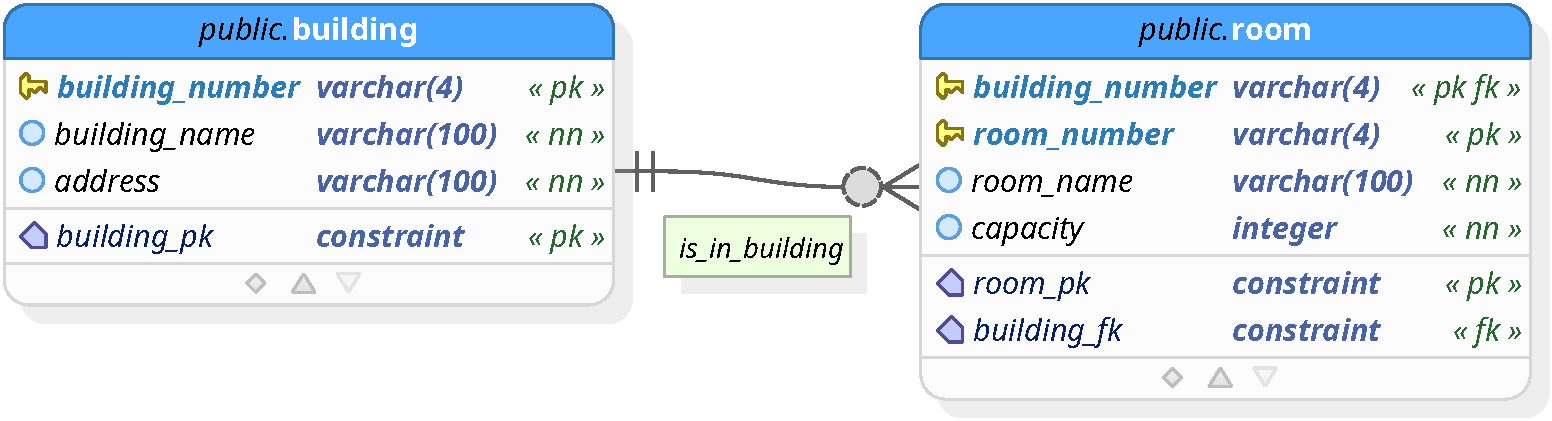
\includegraphics[width=0.56\linewidth]{\currentDir/fixed2nf}%
%
\caption{A different approach to \cref{fig:violation2nf:model} that no longer violates the \pgls{2NF}. %
The columns that only depend on the \sqlil{building_number} have been extracted into their own table.}%
\label{fig:fixed2nf}%
\end{figure}%
%
\gitExec{\databasesCodeRepo}{.}{_scripts_/postgres.sh normalization/2nf/fixed/generated_sql 01_fixed_database_2001.sql}%
%
\gitSQL{\databasesCodeRepo}{normalization/2nf/fixed/generated_sql/04_public_building_table_5080.sql}{2nf:fixed:04_public_building_table_5080}{The generated \sql\ code for creating the table~\sqlil{building}.}%
\gitExec{\databasesCodeRepo}{.}{_scripts_/postgres.sh normalization/2nf/fixed/generated_sql 04_public_building_table_5080.sql fixed}%
%
\gitSQL{\databasesCodeRepo}{normalization/2nf/fixed/generated_sql/03_public_room_table_5071.sql}{2nf:fixed:03_public_room_table_5071}{The generated \sql\ code for creating the table~\sqlil{room}.}%
\gitExec{\databasesCodeRepo}{.}{_scripts_/postgres.sh normalization/2nf/fixed/generated_sql 03_public_room_table_5071.sql fixed}%
%
\gitSQL{\databasesCodeRepo}{normalization/2nf/fixed/generated_sql/05_public_room_building_fk_constraint_5099.sql}{2nf:fixed:05_public_room_building_fk_constraint_5099}{The generated \sql\ code for creating the foreign key constraint linking the rows in table~\sqlil{room} to the rows in table~\sqlil{building}.}%
\gitExec{\databasesCodeRepo}{.}{_scripts_/postgres.sh normalization/2nf/fixed/generated_sql 05_public_room_building_fk_constraint_5099.sql fixed}%
%
\gitSQL{\databasesCodeRepo}{normalization/2nf/fixed/insert.sql}{normalization:2nf:fixed:insert}{%
Inserting the very same data as in \cref{lst:normalization:2nf:violation:insert} into the tables~\sqlil{building} and \sqlil{room}.}%
\gitExec{\databasesCodeRepo}{.}{_scripts_/postgres.sh normalization/2nf/fixed insert.sql fixed}%
%
\gitSQLAndOutput{\databasesCodeRepo}{normalization/2nf/fixed}{delete.sql}{fixed}{}{}{postgres.sh}{normalization:2nf:fixed:delete}{%
First, we select a list of all buildings from the \db, which yields 4~buildings. %
(Notice that we do no longer need the \sqlilIdx{DISTINCT} keyword, since each building ist listed only once in tale~\sqlil{building}.) %
Then we delete the two offices 904a and 904b of Building~53 from our \db. %
This no longer causes a deletion anomaly, as the data of Building~53 is not deleted. %
So when we select the list of all buildings again, it is still there. %
This is different from the situation in \cref{exec:normalization:2nf:violation:delete}, where it disappeared.}%
%
\gitSQLAndOutput{\databasesCodeRepo}{normalization/2nf/fixed}{update.sql}{fixed}{}{}{postgres.sh}{normalization:2nf:fixed:update}{%
We want to see all rooms in South Campus~2. %
Compared to \cref{lst:normalization:2nf:violation:update}, the query is more complex as we now need an \sqlilIdx{INNER JOIN}. %
Due to the inconsistent spelling~(South Campus~II vs.\ South Campus~2), the first query finds nothing. %
We then run a modified query, which gives us all the rooms. %
We can also fix the table~\sqlil{building} by updating the corresponding rows, after which the first query also works correctly. %
Notice that here, only one row is updated. %
In \cref{exec:normalization:2nf:violation:update}, two rows were affected.%
}%
%
\gitSQLAndOutput{\databasesCodeRepo}{normalization/2nf/fixed}{update2.sql}{fixed}{}{}{postgres.sh}{normalization:2nf:fixed:update2}{%
We want to change the name of Building~36 to \inQuotes{Computer Science Building.} %
Different from the situation in \cref{exec:normalization:2nf:violation:update2}, only a single row needs to be changed.%
}%
%
\gitExec{\databasesCodeRepo}{.}{_scripts_/postgres.sh normalization/2nf/fixed cleanup.sql}%
%
So let us normalize the \db\ from the previous section into the \pgls{2NF}.
Back then, we had composite primary key consisting of the \sqlil{building_number} and \sqlil{room_number} in our table~\sqlil{building_room}.
However, the columns \sqlil{building_name} and \sqlil{address} only depend on \sqlil{building_number}.
This has led to several anomalies.
To achieve normalization into the \pgls{2NF}, we have to separate the columns \sqlil{building_name} and \sqlil{address} into an own table.
We will call this table~\sqlil{building}.
Of course, it also needs a primary key, which will be~\sqlil{building_number}.

We rename the rest of the table~\sqlil{building_room} to \sqlil{room}.
Each row now, indeed, just represents a single room in a building.
This table still has the composite primary key~\sqlil{building_number} and~\sqlil{room_number}, as well as the fields~\sqlil{room_name} and~\sqlil{capacity}.
Clearly, both non-key fields are functionally dependent on the primary key.
As a bonus additionally to satisfying the \pgls{2NF}, this design, illustrated in~\cref{fig:fixed2nf}, represents our original conceptual model given in \cref{fig:erdRoom2} much better.

We now implement this design using \sql.
\Cref{lst:2nf:fixed:04_public_building_table_5080,lst:2nf:fixed:03_public_room_table_5071,lst:2nf:fixed:05_public_room_building_fk_constraint_5099} create the tables~\sqlil{building} and~\sqlil{room} and establish the foreign key constraint linking each row of table~\sqlil{room} to one row of table~\sqlil{building}.

We can now insert the exactly as same data as in the last section into this \db.
\Cref{lst:normalization:2nf:fixed:insert} therefore needs two~\sqlilIdx{INSERT INTO} statements.
First we store all the building data into the table~\sqlil{building}.
Then we store the information about the rooms into table~\sqlil{room}.
We immediately notice that now, there is much less redundancy.
The data about each building is stored exactly once, whereas before, we needed to store it for each room.
Since we need to write data much less often, it becomes much less likely to make errors.
And if we make errors, they are easier to spot, since there are fewer records that we would need to check.

In \cref{lst:normalization:2nf:fixed:delete}, we now reproduce the example from \cref{lst:normalization:2nf:violation:delete}.
We first want to get a list of all buildings.
This can be done using the query \sqlil{SELECT building_number, building_name FROM building;}.
Notice that, compared to \cref{lst:normalization:2nf:violation:delete}, we do no longer need to write the \sqlilIdx{DISTINCT} keyword.
In the table~\sqlil{building_room}, each building number and name could appear several times, as they were stored for each room.
However, in our new table~\sqlil{building}, they can only appear once.
Hence, the deletion of duplicate rows, performed by \sqlilIdx{DISTINCT}, is now no longer necessary.
Anyway, our query gives us a list of four buildings.

We then again delete the two offices~904a and~904b of Building~53 using a \sqlilIdx{DELETE} query.
The \sqlilIdx{RETURNING} statement in the query again shows us the two deleted offices.
Back in the previous section, deleting these rows also deleted all information about Building~53.
This \cref{def:deletionAnomaly} was caused by our violation of the \pgls{2NF}.
Back then, issuing the \sqlilIdx{SELECT} query again would yield only three buildings.
However, as you can see in \cref{exec:normalization:2nf:fixed:delete}, this does not happen now.
The building records are independently stored in table~\sqlil{building} and not affected by the deletion of rows in table~\sqlil{room}.
All four building records remain.

In \cref{lst:normalization:2nf:fixed:update}, we reproduce the example from \cref{lst:normalization:2nf:violation:update}:
We want to get a list of all rooms available in South Campus~2.
When comparing the queries necessary to achieve this between the two listings, we notice the \emph{drawback} of the~\pgls{2NF}.
We now have a more complex query.
Before, the building address was stored together with the room number in a single row.
This is no longer the case.
The room information is now stored in table~\sqlil{room}.
However, the building address is stored in table~\sqlil{building}.
If we want to find out whether a room is in South Campus~2, we must combine the data from these two tables.
An \sqlilIdx{INNER JOIN} does the trick.
The primary key of table~\sqlil{building} is \sqlil{building_number}.
The \sqlil{building_number} is a foreign key of table~\sqlil{room}~(and also part of that table's primary key).
So the join condition \sqlil{room.building_number = building.building_number} allows us to find the right row in table~\sqlil{building} for each row in table~\sqlil{room}.

So we execute this slightly more complex query.
We are baffled to notice that this yields no result at all.
There are no rooms in South Campus~2?
OK, we deleted the two rooms in Building~53, which were in South Campus~2.
So they are gone.
But there still should be Building~36 with its three rooms.

Upon closer inspection of the data we inserted in \cref{lst:normalization:2nf:fixed:insert}, we realize that we made the mistake to write the address of Building~36 as~\emph{South Campus~II} instead of~\emph{South Campus~2}.
Since we only store the building record once, this affected all rooms belonging to it.

This problem can be fixed exactly in the same ways as back in \cref{lst:normalization:2nf:violation:update}.
We can either just expand our selection condition to also include South Campus~II.
This works, but it also is a bit unsatisfying.
Should we really leave inconsistent data in our \db?

No.
Of course not.
We decide to fix this by applying \sqlil{SET address = 'South Campus 2'}\sqlIdx{UPDATE} to all rows of table~\sqlil{building} where \sqlil{address = 'South Campus II'}.
We also return the number of the building that is affected by this update.
As the result, we see that a single row in the table~\sqlil{building} is changed.
Back in \cref{lst:normalization:2nf:violation:update}, two rows needed to be changed.
That was an example of the update anomaly.
After the update, the first query works as expected.

A clearer example of the update anomaly that occurs when the \pgls{2NF} is violated was given in \cref{lst:normalization:2nf:violation:update2}.
When we wanted to change the name of Building~36 from \emph{CS Teaching Building} to \emph{Computer Science Building}, we needed to update three rows.
We wanted to change one piece of information, but three changes were actually required.
Now that we observe the \pgls{2NF}, doing the same thing in \cref{lst:normalization:2nf:fixed:update2} only affects a single row in table~\sqlil{building}.
The anomaly has disappeared.%
%
\FloatBarrier%
\endhsection%
%
